%
% introbeispiel.tex
%
% (c) 2020 Prof Dr Andreas Müller, Hochschule Rapperswil
%
\begin{frame}
\frametitle{DGL $\Leftrightarrow$ Minimalproblem}
\vspace{-15pt}
\begin{columns}[t]
\begin{column}{0.48\hsize}
\begin{block}{Schwingende Saite: DGL}
Eigenwertproblem: finde $u(x)$ derart, dass
\begin{align*}
u''(x) &= \lambda u(x), \quad x\in(0,1) \\
u(0) &= u(1) = 0
\end{align*}
\end{block}
\end{column}
\begin{column}{0.48\hsize}
\uncover<2->{%
\begin{block}{Äquivalentes Minimalproblem}
Finde $u(x)$ derart, dass 
\[
I(u)
=
\int_0^1 u'(x)^2 + \lambda u(x)^2 \,dx
\]
\ifthenelse{\boolean{presentation}}{\only<-11>{minimal}}{}\only<12->{stationär} ist.
\end{block}}
\end{column}
\end{columns}
\uncover<3->{%
\begin{proof}[Beweis (``Ableiten---Nullsetzen'')]
Für jede Variation $u(x) \to u(x) + \varepsilon h(x)$, mit $h(0)=h(1)=0$
\\
\begin{tikzpicture}[>=latex,thick]
\node at (0,0) [right] {
$\displaystyle
{\color{white}\bigg]_0^1}
\uncover<6->{0=}
\uncover<5->{\frac{d}{d\varepsilon}}
I(\varepsilon) 
\uncover<6->{\bigg|_{\varepsilon=0}}
=
\ifthenelse{\boolean{presentation}}{
\only<4>{%
\int_0^1 (u(x)+\varepsilon h(x))^{\prime 2} +\lambda (u(x)+\varepsilon h(x))^2\,dx
}%
\only<5-6>{%
\int_0^1 2 u'(x)h'(x) \only<-5>{+ 2\varepsilon h'(x)^2} \,dx 
+
\lambda
\int_0^1 2u(x)h(x) \only<-5>{+ 2\varepsilon h(x)^2}\,dx
}
\only<7>{\biggl[ 2u'(x)h(x)\biggr]_0^1
-
\int_0^1 2u''(x) h(x)\,dx
+\lambda\int_0^1 2u(x)h(x)\,dx}}{}
\only<8->{
-
\int_0^1 \uncover<-8>{2}(u''(x)-\lambda u(x) )h(x)\,dx}
\only<10->{\qquad\Leftrightarrow\qquad u''(x)=\lambda u(x)}
$};
\uncover<6->{
\node[color=blue] at (0.4,-1) [right] {$I(u)$ \ifthenelse{\boolean{presentation}}{\only<-11>{minimal}}{}\only<12->{stationär}\strut};
}
\uncover<11->{
\node[color=blue] at (13.2,-1) [left] {Differentialgleichung\strut};
}
\end{tikzpicture}
\\[3pt]
\end{proof}}
\vspace{100pt}
\end{frame}
